\section{F4RM: Feature-Restricted Round-Robin Random Mapping} \label{sec:f4rm}

\subsection{Preliminaries: WiSARD and Thermometer Encoding}
\label{sec:f4rm-prelim}

WiSARD~\cite{aleksander1984wisard} classifies binary inputs through lookup tables called RAMs (Figure~\ref{fig:wisard-pipeline}). A model with $M$ classes contains $M$ discriminators, one per class; each discriminator holds the same $R$ RAMs, and each RAM stores a counter for every address it has seen. Training is a single pass that increments the correct-class RAM counters; inference queries all discriminators, sums each one's RAM counters, and predicts the highest-scoring class. Real implementations use sparse storage, so memory grows with the number of distinct patterns observed rather than with $2^a$~\cite{susskind2022bthowen}. A standard refinement called bleaching~\cite{grieco2010producing} suppresses single-example memorization by requiring repeated observation of an address before its counter contributes; we use bleaching threshold $b = 1$ throughout, matching the \texttt{wisardpkg}~\cite{wisardpkg} default. The decision pipeline involves no arithmetic beyond integer addition, no floating-point, and no gradient, which is what makes WiSARD attractive at the edge.

Real-valued inputs must be binarized before WiSARD can process them. We use thermometer encoding, the de facto standard in the WiSARD literature. A thermometer encoder of size $t$ maps $x \in [0,1]$ to the binary vector $[b_1,\ldots,b_t]$ with $b_i = 1$ iff $i/t \leq x$. The encoding preserves a monotonic correspondence between value distance and Hamming distance, two values $x_1, x_2$ produce codes differing in $t \cdot |x_1 - x_2|$ bits, a property that binary or Gray codes~\cite{gray1953pulse} lack. We use the \emph{distributive} variant~\cite{lima2020distributive}, placing each threshold at a quantile of the training distribution. Features are min-max scaled on the training set before encoding.

An input with $n$ real features at thermometer size $t$ yields a binary vector of length $n \cdot t$, partitioned into $R = \lceil n \cdot t / a \rceil$ disjoint RAM chunks of size $a$. The assignment of the $n \cdot t$ bits to RAM positions, fixed at initialization, shared across discriminators, is the \textbf{mapping} that F4RM redefines.

\subsection{Standard Random Mapping and Its Limitations}
\label{sec:f4rm-cost}

Standard WiSARD uses a uniformly random permutation as its mapping, conventional, requiring no design effort, and not previously challenged on accuracy grounds. But it treats all $n \cdot t$ bits as interchangeable, ignoring a structural property of thermometer-encoded inputs that can be exploited for free: the $t$ bits of one feature form a contiguous block of 1s followed by 0s, so they take only $t+1$ distinct values instead of $2^t$. When random mapping places multiple bits from the same feature into the same RAM, this redundancy imposes two simultaneous costs. \emph{Feature-coverage loss}: a RAM receiving two bits from feature $f$ forces another RAM to receive one fewer, and in the limit leaves some RAM blind to $f$. \emph{Effective-capacity loss}: $c$ bits from a single feature jointly produce $c+1$ patterns instead of $2^c$, shrinking the RAM's usable address space by a factor of $(c+1)/2^c$, down to $3/4$ at $c=2$ and $1/2$ at $c=3$.

Both costs scale with the frequency of same-feature collisions, governed by the ratio $a/n$: when $a/n \ll 1$ collisions are rare by chance and both costs are negligible; when $a/n \geq 1$ the pigeonhole principle guarantees at least one collision per RAM, and the expected count grows with the ratio. The ratio $a/n$ is therefore the natural axis along which any mapping-rule benefit must be measured, and it returns throughout the analysis that follows.

\subsection{The F4RM Rule}
\label{sec:f4rm-rule}

F4RM resolves both costs through a single rule on the mapping: each RAM should read bits from the maximum possible number of distinct features, and when the address size forces some feature to contribute multiple bits to a single RAM, those multi-bit contributions should be spread evenly across RAMs. When $a \leq n$, every RAM reads $a$ distinct features, one bit each; when $a > n$, every RAM reads every feature at least once with the extras spread evenly.

A round-robin construction realizes this rule: at each step it picks the next feature (in a seeded shuffled order), then its next unassigned thermometer bit (in an independently shuffled order), and places the bit in the RAM with the fewest bits from that feature so far (ties broken by RAM load). The construction runs in $O(n \cdot t)$ time, is data-independent and seed-deterministic, and preserves stochastic diversity along the only dimension F4RM does not constrain, thermometer-level placement, so different seeds yield different valid F4RM mappings (exploited by F4RMS in Section~\ref{sec:f4rm-extensions}). Figure~\ref{fig:f4rm-vs-random} illustrates the rule on a 4-feature toy example.

\begin{figure}[ht!]
 \centering
 \begin{subfigure}[b]{0.46\textwidth}
 \centering
 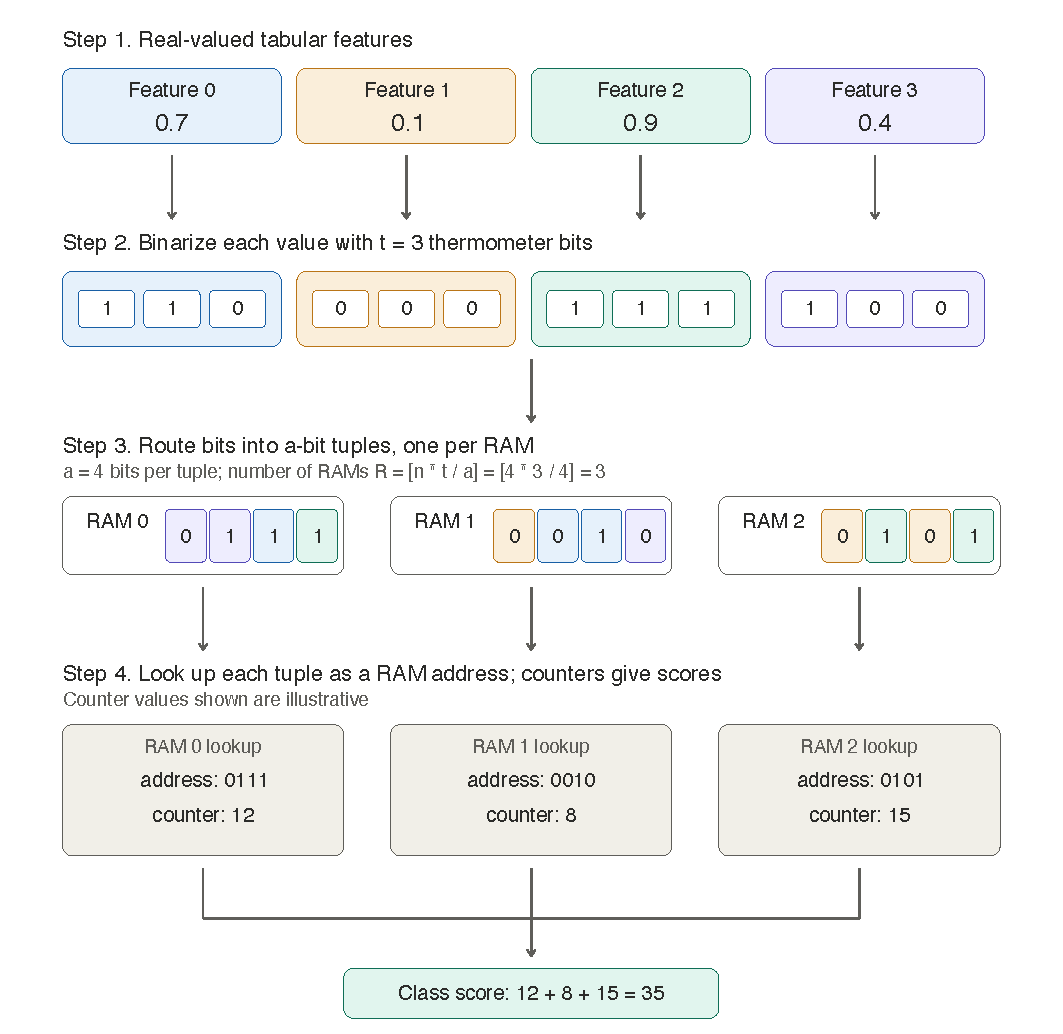
\includegraphics[width=\linewidth]{figures/wisard_primer_pipeline.pdf}
 \caption{WiSARD pipeline (one discriminator): thermometer-encode features, route bits to fixed-size tuples by the mapping, look up each tuple in its RAM, sum counters for the class score.}
 \label{fig:wisard-pipeline}
 \end{subfigure}
 \hfill
 \begin{subfigure}[b]{0.5\textwidth}
 \centering
 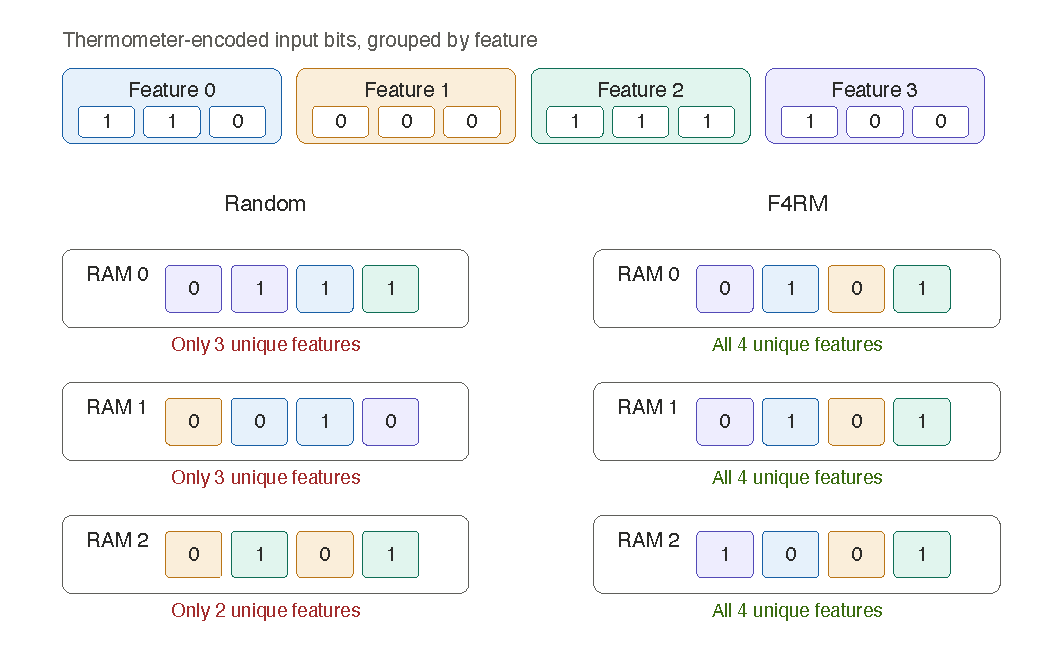
\includegraphics[width=\linewidth]{figures/f4rm_vs_random_mapping.pdf}
 \caption{F4RM versus default random mapping on a small example: 12 thermometer bits from 4 features routed into 3 RAMs of size 4. Random clusters bits from the same feature in some RAMs; F4RM guarantees every RAM reads from every feature.}
 \label{fig:f4rm-vs-random}
 \end{subfigure}
 \caption{(\subref{fig:wisard-pipeline}) The WiSARD architecture F4RM operates on. (\subref{fig:f4rm-vs-random}) The mapping rule F4RM imposes, contrasted with the standard random permutation.}
 \label{fig:wisard-and-f4rm}
\end{figure}

Figure~\ref{fig:mapping-and-decay} shows the same mechanism on real data: F4RM produces visibly uniform feature coverage on Seeds where random mapping clusters same-feature bits (\subref{fig:mapping-seeds}), and its accuracy advantage on EEG Eye State decays predictably as thermometer size $t$ raises capacity at fixed $a, n$ (\subref{fig:capacity-decay-eeg}), confirming F4RM improves information efficiency rather than adding capacity, and remaining ahead throughout the sweep.

\begin{figure}[ht!]
 \centering
 \begin{subfigure}[b]{0.6\textwidth}
 \centering
 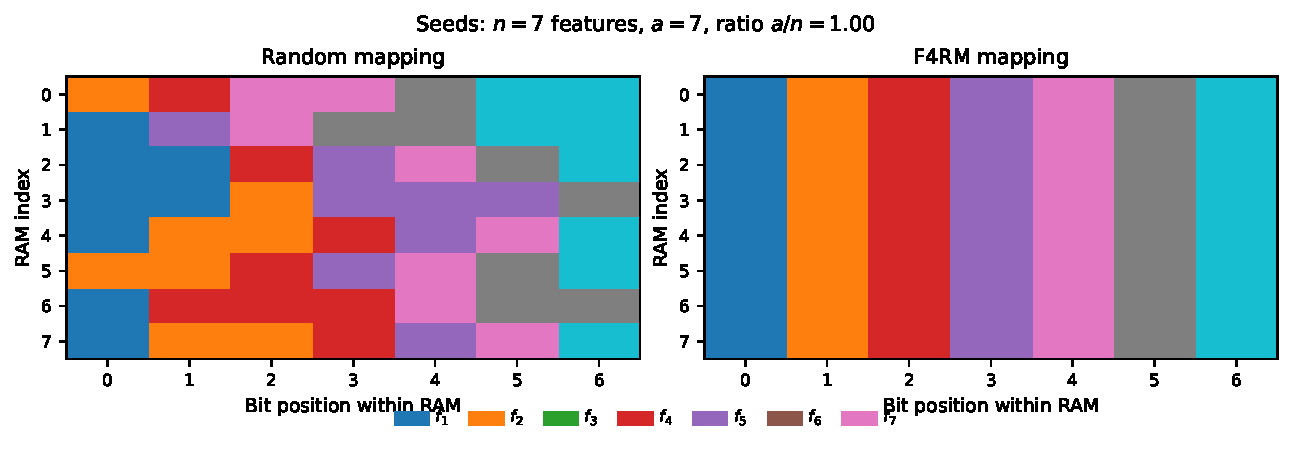
\includegraphics[width=\linewidth]{figures/mapping_seeds.pdf}
 \caption{Random vs.~F4RM mapping on Seeds ($n=7$, $a=7$, $t=8$). Random clusters same-feature bits and skips features in some RAMs; F4RM places one bit from every feature in every RAM, producing perfect vertical stripes.}
 \label{fig:mapping-seeds}
 \end{subfigure}
 \hfill
 \begin{subfigure}[b]{0.36\textwidth}
 \centering
 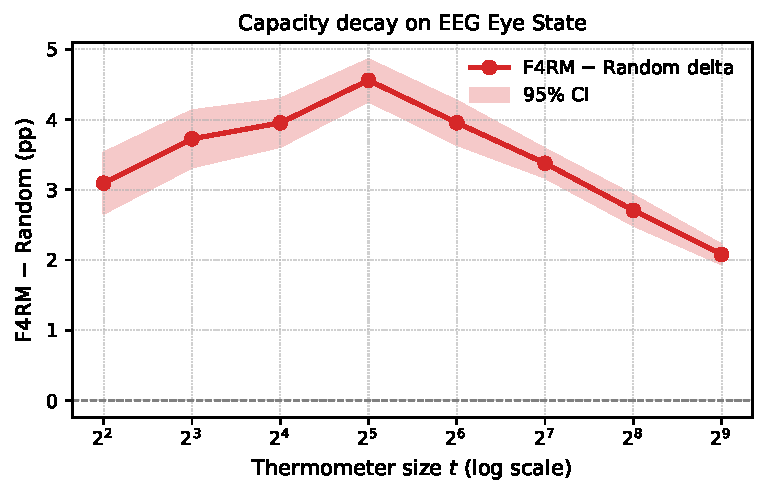
\includegraphics[width=\linewidth]{figures/capacity_decay_eeg.pdf}
 \caption{Capacity decay on EEG Eye State: F4RM$-$Random delta peaks at $t=32$ ($+4.6$~pp), decays at higher $t$.}
 \label{fig:capacity-decay-eeg}
 \end{subfigure}
 \caption{F4RM mechanism on real data: uniform feature coverage (\subref{fig:mapping-seeds}) and a predictable capacity-dependent advantage (\subref{fig:capacity-decay-eeg}).}
 \label{fig:mapping-and-decay}
\end{figure}

\subsection{Address-Size Selection}
\label{sec:f4rm-address}

WiSARD's behavior depends strongly on the address size $a$, and the choice of $a$ has an established trade-off. Too small, and each RAM captures too narrow a bit pattern to support useful discrimination, the model under-fits. Too large, and the nominal address space $2^a$ exceeds what the training set can populate; most addresses remain empty, and the RAMs memorize training samples rather than generalize~\cite{susskind2022bthowen}. The standard approach in WiSARD work is per-dataset hyperparameter sweep~\cite{susskind2022bthowen}, in which $a$ and $t$ are tuned jointly on a validation set to maximize accuracy.

Per-dataset sweeps confound a structural comparison of mappings: selecting hyperparameters per-mapping risks attributing to the mapping what is really a selection effect. To evaluate F4RM against random mapping fairly, we adopt a principled default rule and apply it identically to both:
\begin{equation}
a = \min\left(2n,\ \lfloor \log_2 m \rfloor\right),
\label{eq:address-size}
\end{equation}
where $n$ is the number of features and $m$ is the number of training samples. Thermometer size is fixed at $t = 8$ for all datasets.

Each term has an independent justification: $2n$ places $a/n = 2$, within the collision-frequent regime where any mapping-level difference is measurable; $\lfloor \log_2 m \rfloor$ caps the address space below the training-set size, since $2^a > m$ leaves most addresses unreachable and RAMs memorize rather than generalize. The rule is not designed to maximize per-dataset accuracy (grid search yields higher peaks); its purpose is to let F4RM's contribution be evaluated without confounding it with hyperparameter selection. The full per-dataset hyperparameter listing is available in the open-source artifact.

\subsection{Compositional Extensions}
\label{sec:f4rm-extensions}

F4RM is a mapping rule, orthogonal to two other axes along which WiSARD has been refined: ensembling~\cite{susskind2023uleen,lusquino2021thesis} and RAM-state storage~\cite{santiago2020bloom,santiago2019thesis,susskind2023uleen}. We define two extensions to verify F4RM composes cleanly with both; neither is a novel architecture in itself.

\textbf{F4RMS} (F4RM enSemble) trains $K$ F4RM WiSARDs at identical $a$ and $t$ but different mapping seeds, aggregating their per-class responses by summation as in ULEEN~\cite{susskind2023uleen}: the ensemble predicts $\hat{y} = \arg\max_c \sum_{k=1}^{K} r^{(k)}_c$. Different seeds produce different valid F4RM mappings (the rule constrains feature placement but leaves thermometer-level placement and feature visit order to randomness), so members differ only in bit-to-RAM assignment. Cost scales linearly with $K$ in raw compute but with no penalty in deployment latency on parallel hardware; Random Subspace Method-style alternatives~\cite{ho1998random,breiman2001random} were tested and found weaker (artifact).

\textbf{F4RM-Cuckoo} pairs the F4RM mapping with cuckoo-filter storage~\cite{fan2014cuckoo} in place of the dense per-class counter table, following Cuckoo WiSARD~\cite{santiago2019thesis} which introduced cuckoo filters as a memory-efficient alternative to Bloom filters~\cite{santiago2020bloom}. F4RM mapping does not modify how RAM state is stored, only which bits each RAM reads, so the substitution requires no change to the F4RM construction or to inference. We evaluate F4RM-Cuckoo separately because storage choice shifts the memory-accuracy operating point, surfacing the low-memory regime where F4RM's collision-free address utilization matters most.
